\section{Bridging unsupervised and supervised}\label{clustering}
After performing dimensionality reduction using kernel PCA and retaining the first 10 principal components, I proceeded to assign labels 
to the resulting data points. Rather than using the true labels, the objective was to cluster the data into 10 groups and then evaluate how well these clusters captured the 
data's underlying structure. To achieve this, I selected agglomerative clustering over the usual K-means for several reasons:
\begin{enumerate}
    \item while K-means performs well with spherical clusters, the transformed data from kernel PCA typically exhibits complex, non-spherical geometries. 
    Agglomerative clustering is better suited to these shapes, as it captures more effectively irregular and overlapping clusters, leading to a closer 
    approximation of the true data structure;
    \item  agglomerative clustering is robust to outliers, making it particularly suitable for a high-dimensional and potentially noisy dataset like ours. 
    Unlike K-means, where outliers influence centroids and lead to distorted assignments, agglomerative clustering is less sensitive to such anomalies, maintaining more reliable clustering results;
    \item agglomerative clustering offered flexibility in the choice of the distance metric. Nevertheless, I still opted to use Euclidean distance specifically to 
    leverage Ward’s linkage, which minimizes the total within-cluster variance (a desirable property in this analysis). Ward’s linkage also tends to produce balanced clusters, 
    aligning with my aim to create clusters that mirror the true, balanced structure of the dataset.
\end{enumerate}

\Cref{fig:sankey_diagram} shows a Sankey diagram representing the flow between the true labels and the cluster assignments, 
making it easier to inspect if there is any relevant correspondence. \Cref{fig:cluster_composition}, instead, shows the composition of each cluster with respect to the true labels, providing an additional, intuitive way to evaluate 
the quality of the clustering procedure.
\begin{figure}[ht]
    \centering
    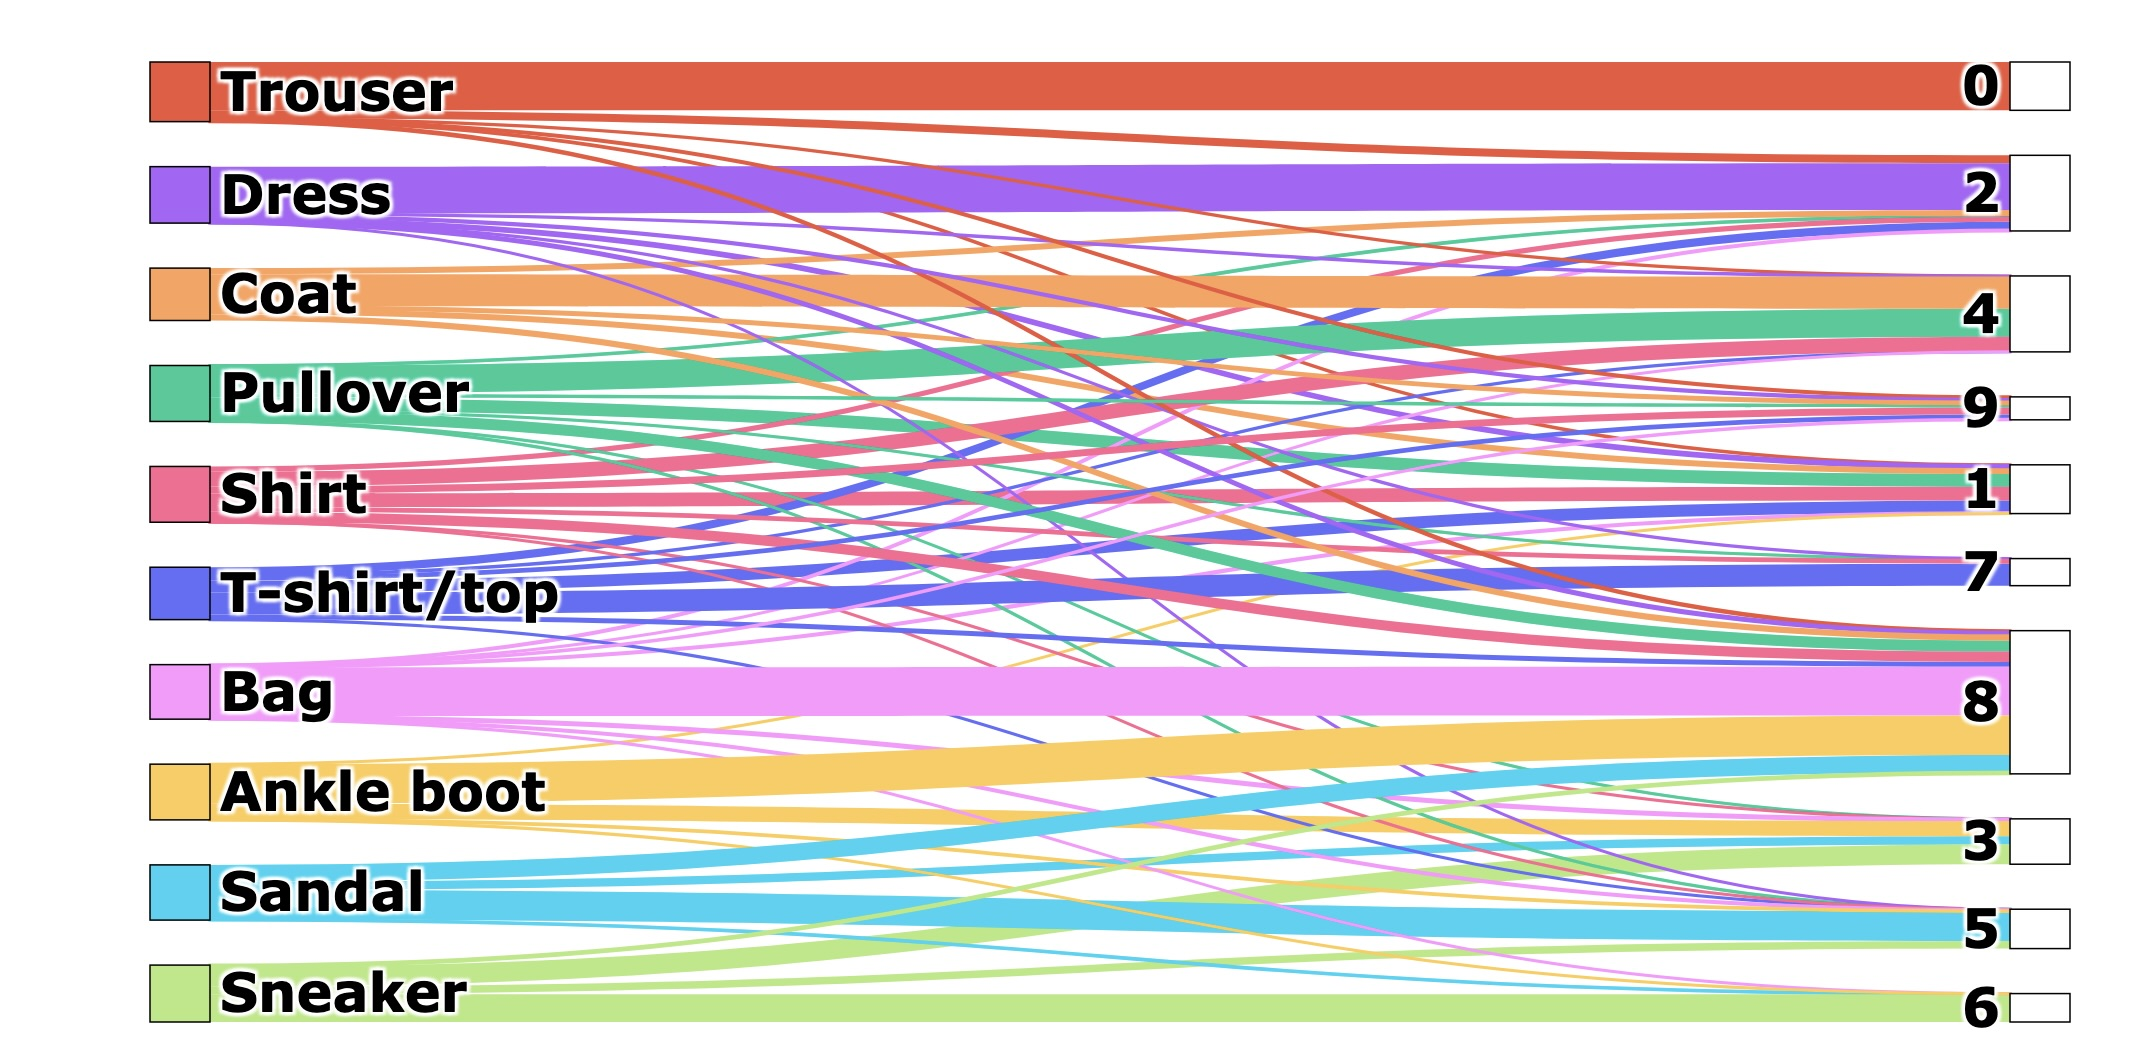
\includegraphics[width=0.62\textwidth]{images/sankey_diagram.png}
    \caption{\footnotesize Sankey diagram}
    \label{fig:sankey_diagram}
\end{figure}

\begin{figure}[ht]
    \centering
    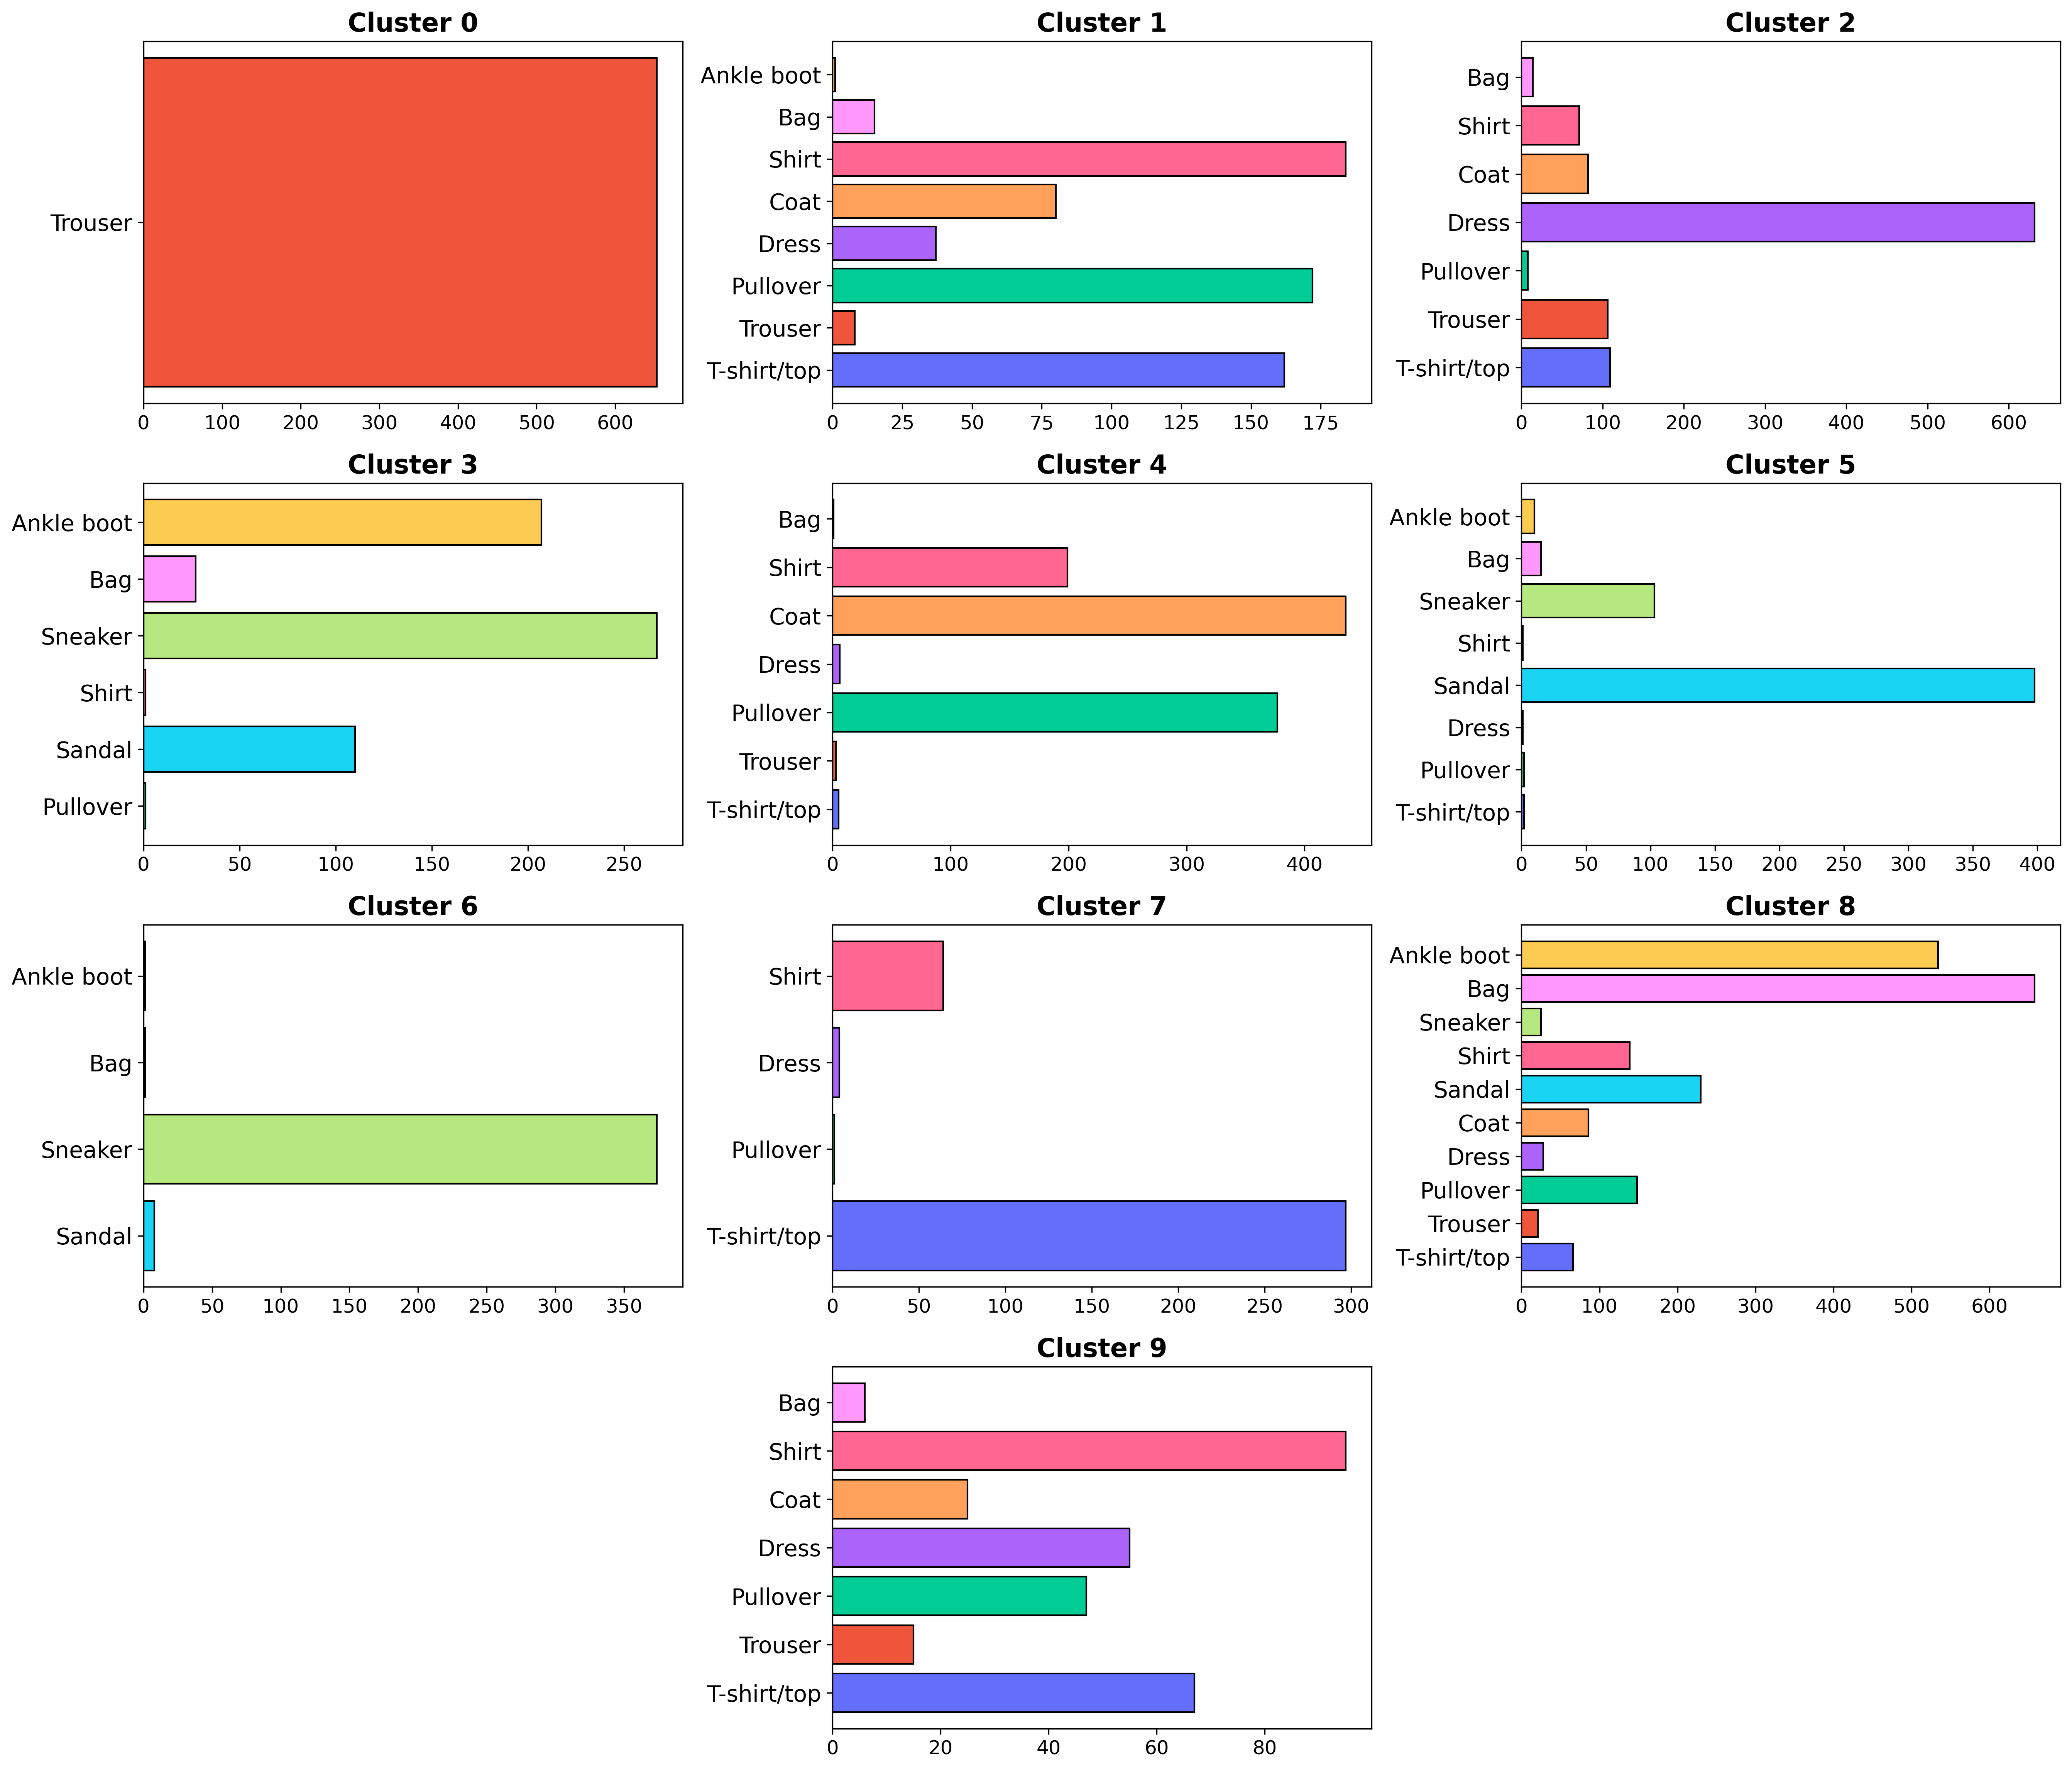
\includegraphics[width=0.85\textwidth]{images/clusters_composition_AC_3x4grid.png}
    \caption{\footnotesize Cluster composition w.r.t. the true labels}
    \label{fig:cluster_composition}
\end{figure}

The cluster composition largely reflects the data geometry discussed in \Cref{data_geometry}. Cluster 0 consists solely of trousers, confirming them as the most 
separable category. Clusters 3, 5, and 6 are instead dominated by footwear, with sneakers being the majority class for clusters 3 and 6 (a redundancy better
discussed in later sections). Clusters 1, 4, and 9 exhibit a balanced mix of shirts, coats, pullovers and T-shirts/tops, underscoring 
the difficulty in distinguishing upper-body clothing items. Cluster 8 shows an interesting deviation: while 
bags appeared well-separated in 2D and 3D projections, it contains a notable proportion of ankle boot samples.
This overlap may be due to actual shared visual features between bags and boots. However, with just 10 components, we may be missing finer details 
that that could improve class separation. This is supported by the spectrum in \Cref{fig:kpa_spectrum}, where the optimal `elbow' 
for component selection likely exceeds 10 components, indicating the need of additional components to improve clustering fidelity.

\begin{figure}[ht]
    \centering
    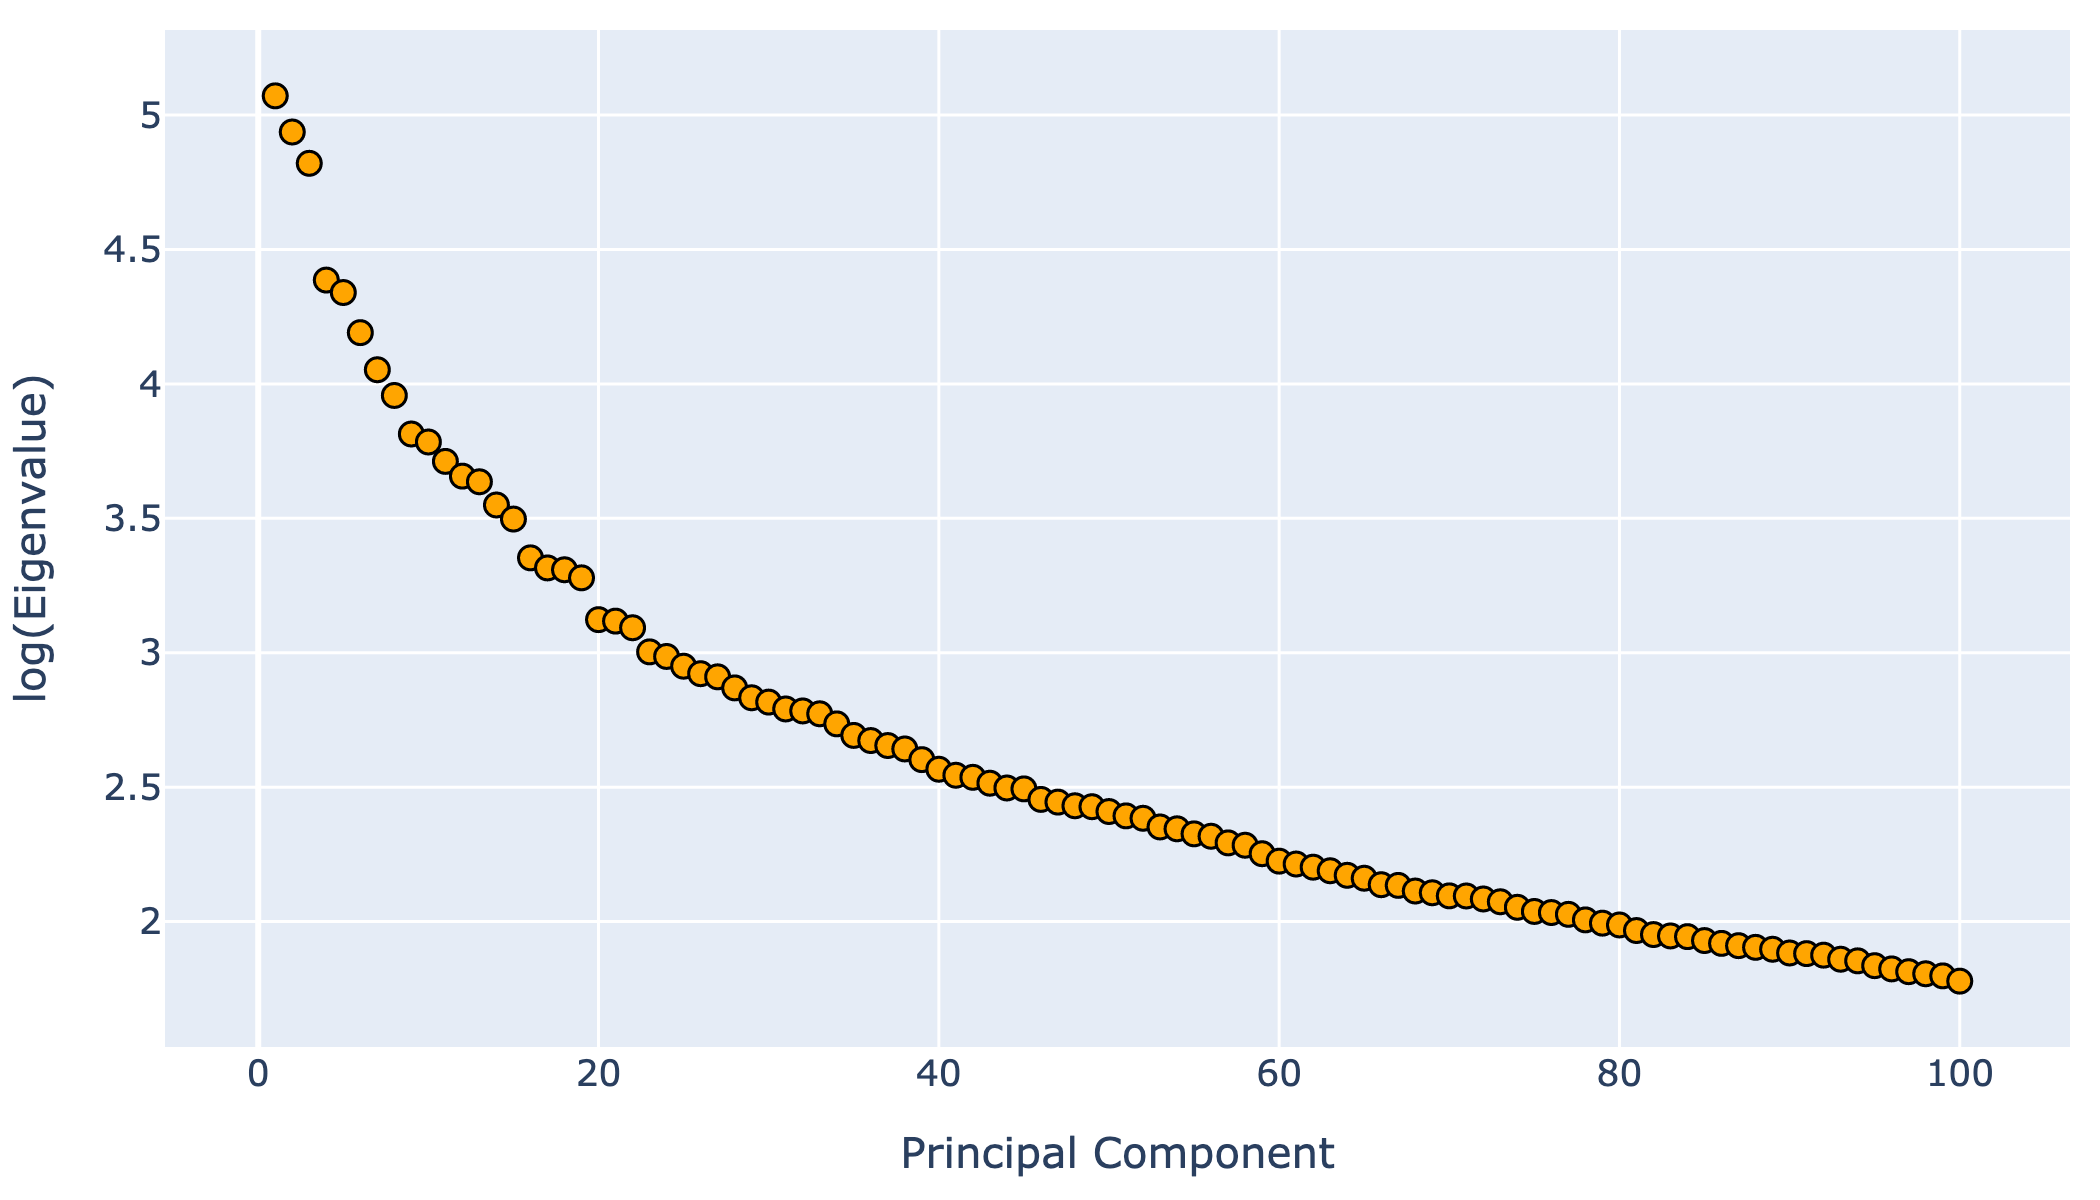
\includegraphics[width=0.5\textwidth]{images/best_kPCA_spectrum.png}
    \caption{\footnotesize Spectrum of the log(eigenvalues) from kernel PCA}
    \label{fig:kpa_spectrum}
\end{figure}
\newpage
To further investigate this, I performed an analysis of the intrinsic dimensionality of the data using the two-NN algorithm 
provided by the \texttt{DADApy} package. The results indicated an intrinsic dimensionality of approximately 15, reinforcing the 
hypothesis that additional components could capture meaningful variation in the data and improve clustering performance. I finally computed 
some quantitative metrics to assess the clustering performance, which are summarized in \Cref{tab:clustering_metrics}.
\begin{table}[h!]
    \centering
    \begin{tabular}{|l|c|}
    \hline
    \textbf{Metric}                  & \textbf{Score}         \\ \hline
    Normalized Mutual Information    & 0.5029                 \\ 
    Adjusted Rand Score              & 0.3257                 \\
    Homogeneity                      & 0.4855                 \\
    Completeness                     & 0.5215                 \\
    V-Measure                        & 0.5029                 \\ \hline
    \end{tabular}
    \caption{Clustering Evaluation Metrics}
    \label{tab:clustering_metrics}
\end{table}
